
\section*{Deployment Options and Security Benefits}

Now that we have seen two commercially deployed, integrated security chips (Titan and T2) and another two research projects where we designed user-attachable dedicated security tokens (\protection and \proximitee), we can compare these solutions based on their deployment options and security benefits. 

\paragraph{Deployment}
Integrated security chips like Titan or T2 can be only issued by major service and platform providers that have the possibility to design and build their own systems. 

\proximitee is an example of a plug-and-play security token that can be attached to the target platform over a standard interface like USB. Obviously, the deployment of security solutions is a feasible option for a larger set of service providers. For example, cloud computing providers can enhance off-the-shelf servers with \proximitee tokens to enable secure, relay-protected attestation on them. Another interesting use case is the secure setup of a permissioned blockchain where every consensus node is hardened with SGX enclaves. The trusted authority that appoints the consensus nodes and bootstraps the chain can issue a \key token to each organization that operates one node.

Also \protection could be deployed as a plug-and-play security module. A user-pluggable token is a good deployment option for web-based online services like e-voting and online banking. Such deployment allows voting authorities and banks to increase the security of their services without restricting the users’ choice of client platform. In medical and industrial domains, an externally-attached \protection module can improve the security of safety-critical systems, even when modifications to the computing platform itself are prohibited due to strict regulations. Alternatively, \protection could be deployed as an integrated security chip such that its functionality is implemented as part of the integrated keyboard, mouse, and display controllers of the computing platform. 

\begin{figure}[t]
    \centering
    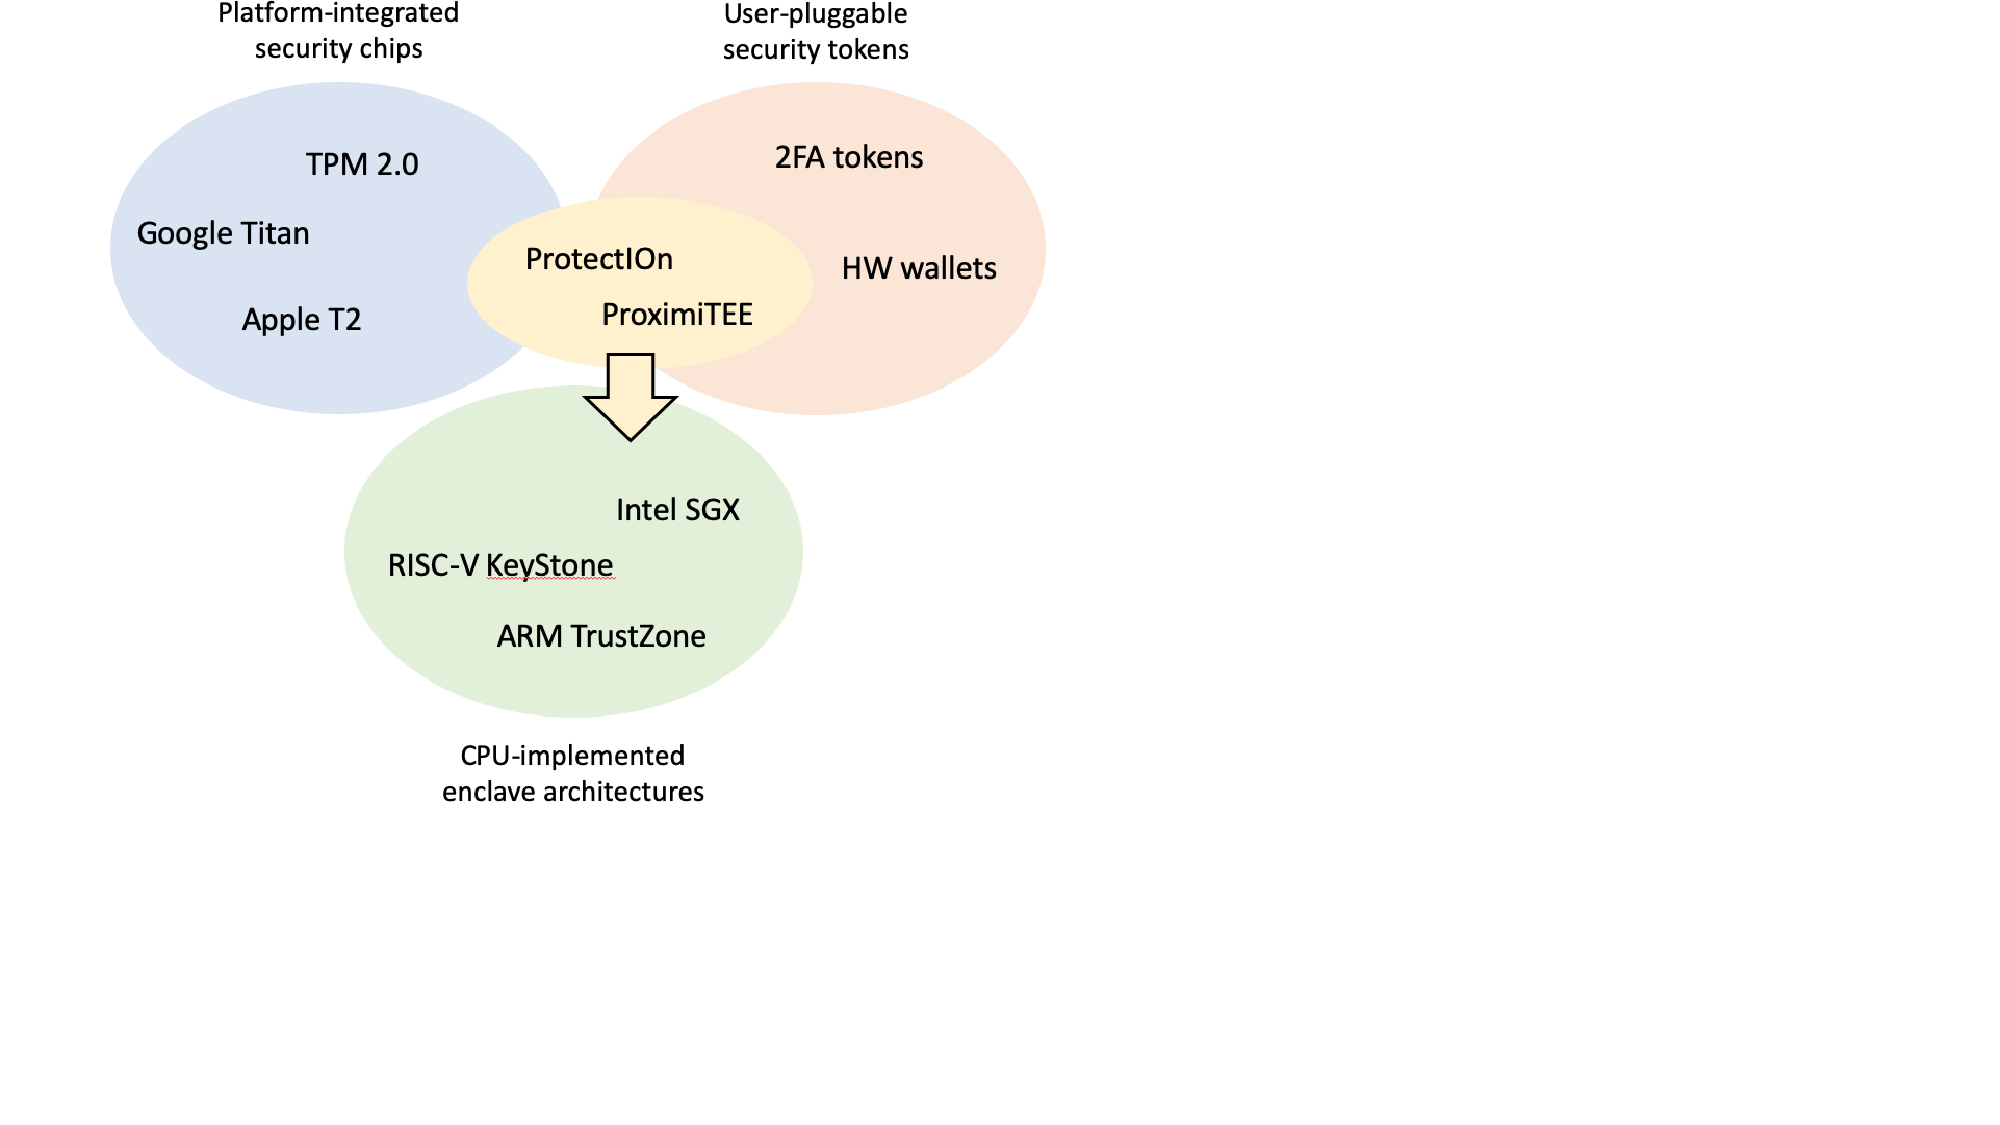
\includegraphics[scale=0.4]{comparison.pdf}
    \caption{Comparison of \protection and \proximitee with respect to the platform-integrated security chips, user-pluggable security tokens and CPU-implemented enclave architecture.}
\label{fig:prototype}   
\end{figure}


\paragraph{Security Benefits}
Titan and T2 are chips that enable security functionality like a secure boot that is missing from enclaves. Thus, the operation of Titan and T2 is largely orthogonal to the operation of enclaves. 

In comparison, \proximitee is a security chip that is designed to work in collaboration with enclaves and improve their security guarantees by enabling secure TEE identification for hardened remote attestation. 

\protection is a solution that can either assist enclaves or operate independently of them. One possible usage for \protection is to enable a trusted path from the user to a local enclave, which can, in turn, can communicate securely with remote servers. In such a deployment, \protection works in collaboration with an enclave and addresses one of the limitations of the SGX architecture --- it's lack of trusted path. Alternatively, \protection could be used to create a trusted path from the user to a remote server without the use of enclaves. Such a deployment option may be beneficial, for example, in cases where the risk of microarchitectural attacks on enclaves is considered too high, and thus, the integrity of the trusted path should not rely on enclave security.


